\documentclass[a4paper,12pt]{scrartcl}
\usepackage[utf8x]{inputenc}
\usepackage[T1]{fontenc} % avec T1 comme option  d'encodage c'est ben mieux, surtout pour taper du français.
%\usepackage{lmodern,textcomp} % fortement conseillé pour les pdf. On peut mettre autre chose : kpfonts, fourier,...
\usepackage[french]{babel} %Sans ça les guillemets, amarchpo
\usepackage{amsmath}
\usepackage{multicol}
\usepackage{amssymb}
\usepackage{tkz-tab}
\usepackage{exercice_sheet}

%\trait
%\section*{}
%\exo{}
%\question{}
%\subquestion{}

\date{}


% Title Page
\title{Utilisation de la calculatrice, Casio Graph 35+}

\author{}

\begin{document}

\maketitle

À noter que dans ce document, on appelle \emph{menu principal} le menu qui permet d'accéder à toutes les fonctions de la calculatrice, c'est-à-dire celui affiché \emph{via} la touche \texttt{MENU}.

\begin{center}
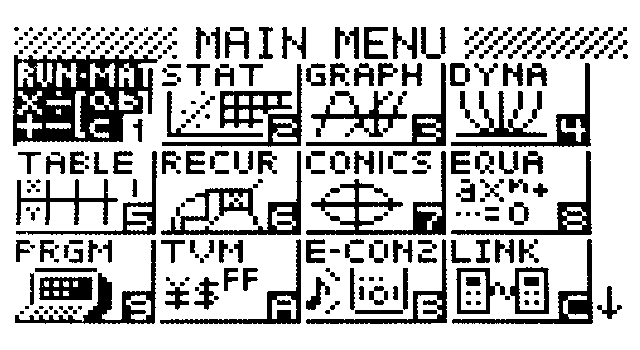
\includegraphics[width=0.7\textwidth]{pics/screen_menuPrincipal.png}
\end{center}

\section{Tracer le graphe d'une fonction $y = f(x)$}

Comme on tracerait le graphe d'une fonction à la main à partir d'un tableau de valeurs, la calculatrice est capable d'afficher la courbe représentative d'une fonction. Pour ce faire:

%$\rightarrow$
\texttt{MENU} ; item \texttt{GRAPH} ; 





%\begin{center}
%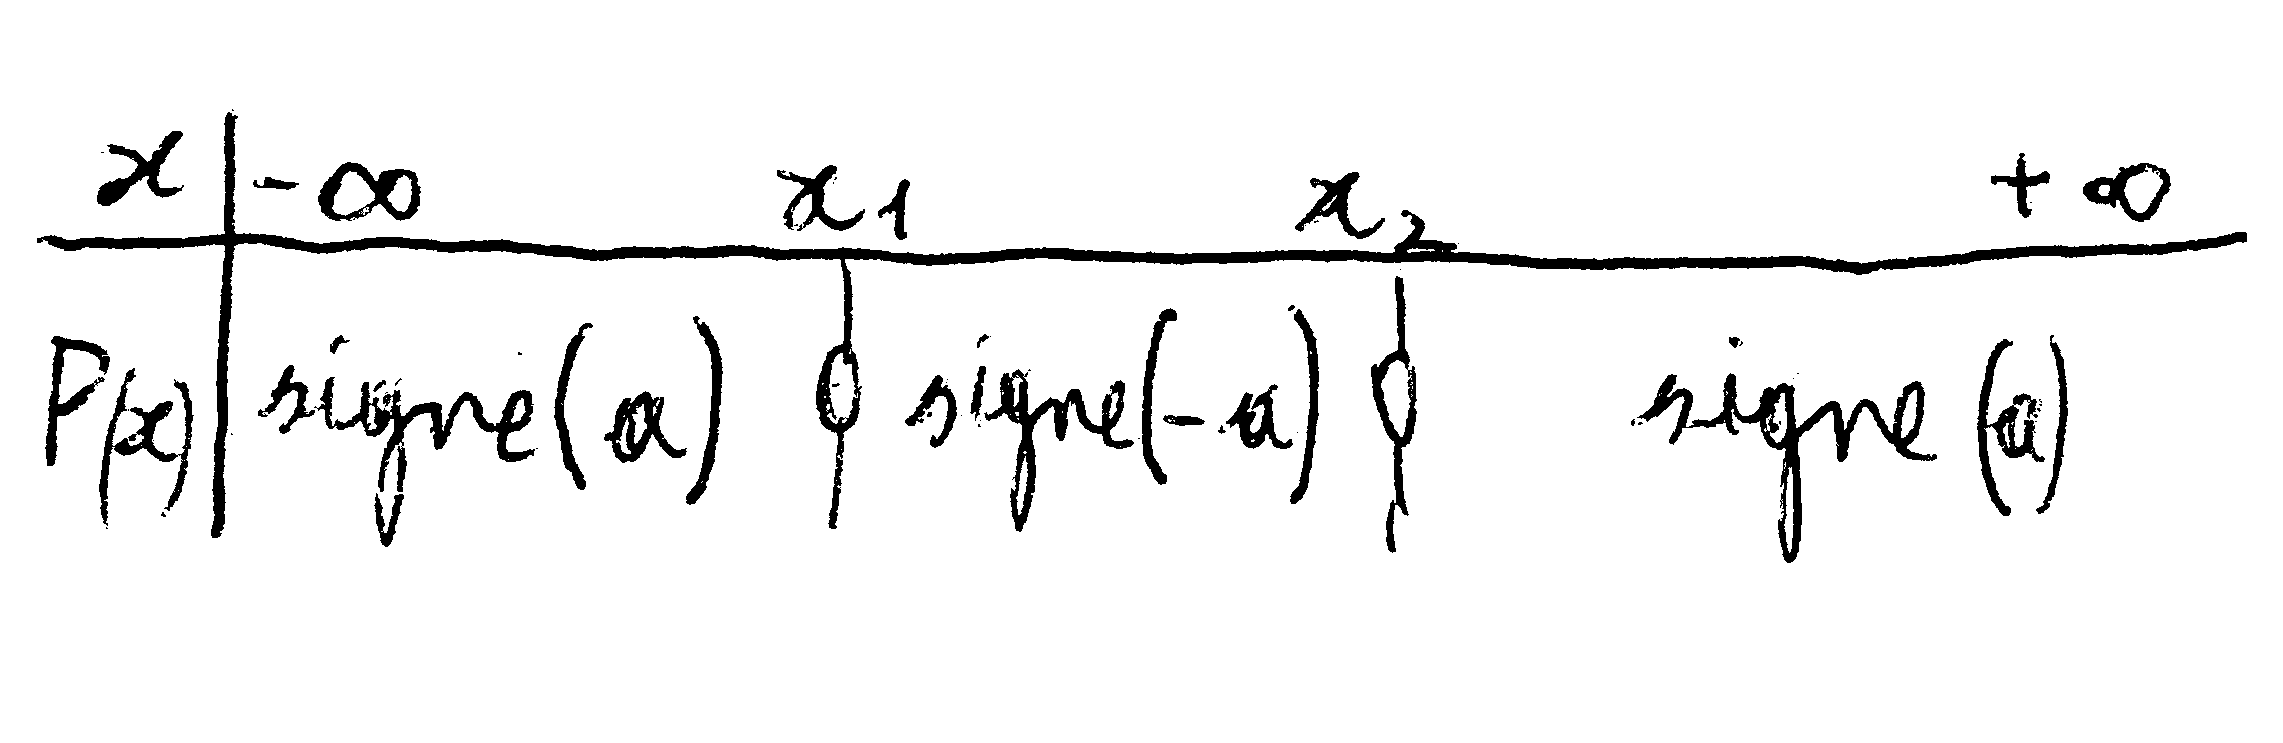
\includegraphics[width=1\textwidth]{pics/3.png}
%\end{center}

\trait

\begin{center}
Fin.
\end{center}

\end{document}
